\documentclass[titlepage, 12pt]{report}

\usepackage[utf8]{inputenc}
\usepackage[T1]{fontenc}
\usepackage[francais]{babel}
\usepackage{listings} %listings for code
\usepackage{graphicx} % can modify title style
\usepackage{titling} % can use pretitle to have a picture on title page
\usepackage{chngcntr} % permits to reset chapter numerization in each part
\usepackage{hyperref} % makes table of contents and list of figures clickable 
\usepackage{makecell} % can create newline in a table cell easily
\usepackage{scrextend}
\addtokomafont{labelinglabel}{\sffamily}
\usepackage{booktabs}

%\hypersetup{colorlinks,citecolor=black,filecolor=black,linkcolor=black,urlcolor=black}

\counterwithin*{chapter}{part}

\addtolength{\oddsidemargin}{-2cm}
\addtolength{\evensidemargin}{-2cm}
\addtolength{\textwidth}{4cm}
\addtolength{\topmargin}{-2cm}
\addtolength{\textheight}{4cm}

\setcounter{secnumdepth}{3}

% Title Page

\pretitle{
	\begin{center}
		\LARGE
		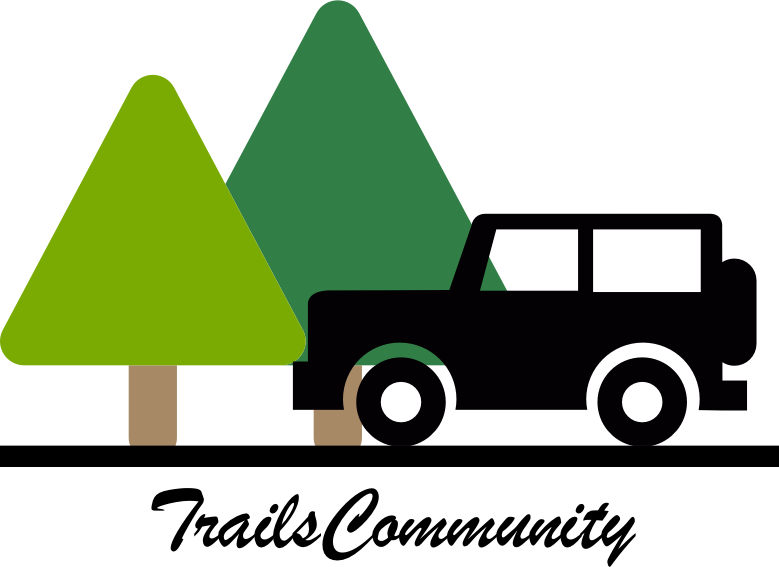
\includegraphics[width=\textwidth]{Images/TrailsCommunity_doc.png}\\[\bigskipamount]
	}
	
	\posttitle{\end{center}}

		\title{Rapport de projet - Assitant Offroad}
		
		\author{BELLANGER Stéphen \and
			MONNIER Ysée \and
			DESHORS Yann}
		\date{Novembre 2016 - Decembre 2016}
		


\begin{document}
	
\maketitle

\tableofcontents

\listoffigures 

\part{Client TrailsCommunity}

\chapter{Introduction}

Cette section fournit  une vue d'ensemble de tout ce qui est inclus dans ce document SRS. De plus, l'objectif de ce document est décrit et une liste de définitions est fournie.

\section{Objectifs}

L'objectif de ce document est de fournir une description détaillée des conditions requises pour l'application TrailsCommunity.
Il illustrera le but et la description complète du développement du système.
Il expliquera également les contraintes du système, l'interface et les intéractions avec les applications externes. Ce document est principalement destiné à être proposé à un client pour son approbation. C'est aussi une référence pour le développement de la première version du système pour l'équipe de développement.

\section{Portée}

TrailsCommunity est une application mobile GPS qui permet au utilisateurs de connaitre en temps réel le positionnement des autres participants d'une activité de pleine air en cours. L'ensemble des activités sont regroupés en type qui seront limmité à une liste pré-défini.
L'application doit être gratuite et simple d'utilisation.
L'organisateur de l'activités devra fournir deux adresses. Une pour le point de départ de l'application et la deuxième pour le point d'arrivé. La création des sessions se fera directement sur l'application mobile.
En outre, le logiciel a besoin à la fois d'Internet et de connexion GPS pour récupérer et afficher les résultats. Tous les systèmes d'informations sont conservés dans une base de données, qui se trouve sur un serveur web. Le logiciel intéragit également avec l'API Google Map qui permettra d'afficher et de tracer les différentes parcours des utilisateurs. De plus, le téléphone doit aussi comprendre un GPS pour pouvoir localiser l'utilisateur à tout moment. 
L'application a également la capacité de représenter à la fois des informations sommaires et détaillées des différentes statistiques de l'utilisateur courant mais aussi des autres participants de la session en cours.

\section{Définitions}
\begin{labeling}{alligator}
	\item [session] une session est une activité disponible dans l’application
	\item [visiteur] personne n’étant pas identifier
	\item [utilisateur] personne identifié à l’application. Il possède les choix de créer ou de rejoindre une session
	\item [organisateur] utilisateur ayant créé une session et pouvant la gérer
	\item [participant] utilisateur qui a rejoint une session
	\item [waypoint] désigne un point de la route a atteindre ou doit avoir lieu un changement de cap
\end{labeling}


\section{Références}
\begin{labeling}{alligator}
	\item [The Institute of Electrical and Electronic Engineer NY USA] IEEE Recommented Practice for SRS, \url{http://www.utdallas.edu/~chung/RE/IEEE830-1993.pdf}
	\item [Chalmers] IEEE standards - SRS Example, 2010, \url{http://www.cse.chalmers.se/~feldt/courses/reqeng/examples/srs_example_2010_group2.pdf}
	\item [Droid5 Informatics Pvt Ltd] androidhive, 2016, \url{http://www.androidhive.info}
	\item [Oracle] Java 8 Documentation, 2016, \url{https://docs.oracle.com/javase/8/docs/api/}
	\item [Google] Android Documentation, 2016, \url{https://developer.android.com/guide}
	\item [James Britt] Ruby Doc, 2016, \url{http://ruby-doc.org}
	\item [Rails Community] Ruby On Rails Documentation, 2016, \url{http://rubyonrails.org}
\end{labeling}

\section{Aperçu}

Le reste de ce document comprend quatres chapitres. Le second fournit une vue d'ensemble de la fonctionnalité du système et de l'intéraction du système avec d'autres systèmes. En outre, le chapitre mentionne également les contraintes du systèmes et les hypothèses sur e produit. Le troisième chapitre fournit la conception et la description du serveur.
Différentes techniques de spécification sont utilisées afin de préciser les exigences plus précisement pour différents publics. Cependant, le lecteur principal sera le correcteur du projet.
Le quatrième chapitre regroupe l'ensemble des annexes du projet. Ce sont en globalité des diagrammes UML. Ils permettent soit une meilleurs finesse de compréhension du système soit, une meilleurs spécification métier du serveur.

\chapter{Description générale}

\section{Perspective du produit}

Ce système ce compose de deux parties : une application mobile et un serveur web.
L'application Android sera utilisé pour la gestion des sessions. Elle permetrta d'afficher en fonction d'une session sélectionner, sur une carte Google map les différentes positions des particiapants.
Le serveur sera tant qu'à lui capable de gérer la récolte et la gestion des données envoyer par l'application.
L'application mobile devra communiquer avec un GPS qui se situe au sein du mobile. Le GPS fournira les emplacements de l'utilisateur et des autres participants. Mais aussi des statistiques sur l'utilisateur courant ainsi que chat pour permettre au différents membres de pouvoir communiquer ensemble.
De manière transparente comme il s'agit d'un produit axé sur la récolte de données, il lui faudra une base de données. La communication avec la base de données se passera via internet.

\section{Fonctions du produit}

Avec l'application mobile, l'utilisateur pourra ce créer un compte utilisateur. Cette première étape va permettre de collecter différentes informations primordiales sur l'utilisateur. 
Après la réalisation de cette première étape, les utilisateurs pourront sélectionner des sessions. Le résultat sera basé sur les sessions que l'utilisateur sélectionne. Il existe 2 types de sessions. Les sessions actives, elle sont encore réalisable et ne sont pas encore clôturées. Cela veut donc dire que leurs dates de fin ne sont pas dépassées. Dans ces sessions, un chat est disponible en temps réel est disponible permettant de communiquer avec tout les participants.
Les sessions clôturé dont l'utilisateur à participé. Elle ce classe dans la section historique qui permet à l'utilisateur courant de pouvoir revisualisé ses anciennes statistiques.
L'application va permet après sélection d'une session, d'afficher une carte Google map ainsi que ensemble de point permetant de décrire le déplacement des différents utilisateurs actif de la session.
De plus, les sessions pourront être directement créée depuis l'application.

\section{Caractéristique de l'utilisateur}

Il existe quatres types d'utilisateurs qui interagissent avec le système : le visiteur, l'utilisateur, le participant et l'organisateur. Chacun de ces trois types d'utilisateurs a une utilisation différente du système affin que chacun ait leurs propres exigences.

Les visiteurs de l'application mobile ne peuvent utiliser TrailsCommunity si il ne sont pas connecter. Cela signifie que le visiteur doit être en mesure de pouvoir créer un compte utilisateur et ainsi pouvoir se connecter.

L'utilisateur qui sont des visiteurs connecter peuvent alors visualiser l'ensemble des sessions actives mais aussi leur historique de session.
De plus, ils peuvent modifier leurs coordonnées personnelles.

Les participants sont des utilisateurs qui ont rejoint une session active, ils peuvent alors ajouter un waypoint et le partager à l'ensemble des participants. Ils peuvent aussi communiquer via un chat en temps réel. De plus, ils peuvent consulter leurs statistiques en cours.

Enfin, les organisateurs sont des utilisateurs qui ont créée une nouvelle session. En effet, ce sont eux dont l'impulsion est venu pour organiser une activités. Ce sont eux qui vont pouvoir faire partager le mot de passe de la session pour pouvoir la rejoindre.

\section{Contraintes}

L'application mobile est limitées au système de navigation GPS du téléphone portable. Comme il existe plusieurs système de fabricants de GPS, la précision n'est pas la même pour chacun d'entre eux. En outre, il peut y avoir une différences de navigation en fonction des téléphone.

La connexion internet est également une contrainte pour l'application. Puisqu'elle récupère les données de la base de données, il est crucial qu'il existe une connexion. De plus en fonction du réseau, il est possible d'avoir une différence du temps de réception des données plus lente.
Il existera une fonctionnalité offline qui permettra entre autre de pouvoir basculer sur un nouveau protocole pour que les utilisateurs puissent continuer à communiquer entre eux. L'ensemble des données récoltés sont alors stockées dans une base de données internet du mobile. Lors de la récupération du réseau internet, l'application va alors recevoir l'ensemble des données collectés en dur et va reprendre son état d'envoi naturel.

\section{Hypothèses et dépendances}

Le produit sera toujours utilisé sur les téléphones mobiles Android qui ont assez de performances. Si le téléphone ne dispose pas de ressources matérielles suffisantes pour l'application. Elle peut ne pas fonctionner comme prévu ou même pas du tout.

Une autre hypothèse est que les composants GPS de tous les téléphones fonctionnent de la même manière. Si les téléphone on un système GPS qu différent des normes, l'application doit être spécifiquement adaptée à chaque interface.

\section{Répartition des besoins}

Dans le cas où le projet est retardé, certaines exigences pourraient être transférées au prochaine version de l'application. Les exigences avec une priorités haute doivent être développé lors du rendu de la première version de l'application.

\chapter{Exigences particulières}

Cette section contient toutes les exigences fonctionnelles et de qualité du système. Il donne une description du système et de toutes ses caractéristiques.

\section{Exigences externe de l'interface}


\end{document}          
